\begin{enumerate}[label=\thesection.\arabic*.,ref=\thesection.\theenumi]
\numberwithin{equation}{enumi}
\item Question-The open loop transfer function of a unity feedback system is given by
\begin{align*}
 G(s)=\frac{\pi e^{-0.25s}}{s}
\end{align*}
in G(s) plane,the Nyquist plot of G(s) passes through the negative real axis at the point
\\*(A)(-0.5,j0)  (B)(-0.75,j0)  (C)(-1.25,j0)  (D)(-1.5,j0)


 

\solution
\begin{align}
G(s)=\frac{\pi e^{-0.25s}}{s}
\end{align}

 Nyquist plot cuts the negative real
Axis at $\omega$ = phase cross over frequency,at phase cross over frequency the phase of nyquist plot becomes -$\pi$ radians.
\
\newline substitute \begin{align}
s=j\omega.\end{align} 
\begin{align}
G(j\omega)&=\frac{\pi}{\omega}(-\sin{0.25\omega}-j\cos{0.25\omega})
\end{align}
\begin{align}
\angle G(j\omega)=-\pi/2 -0.25\omega.
\end{align}
\begin{align}
\angle G(j\omega)|_{\omega=\omega_{pc}}=-\pi
\end{align}
by solving for $\omega$ we get $\omega_{pc}=2\pi$.
\
\newline magnitude at any point is\begin{align}
X=|G(j\omega)|=\frac{\pi}{\omega}.    
\end{align} 
\
\newline substituting $\omega=2\pi$ in magnitude equation we get X=0.5.
\\
\newline so it intersects at (-0.5,0j) so answer is A.
\\
\newline we can verify with the following plot that it intersects at (-0.5,0j)
\begin{figure}
  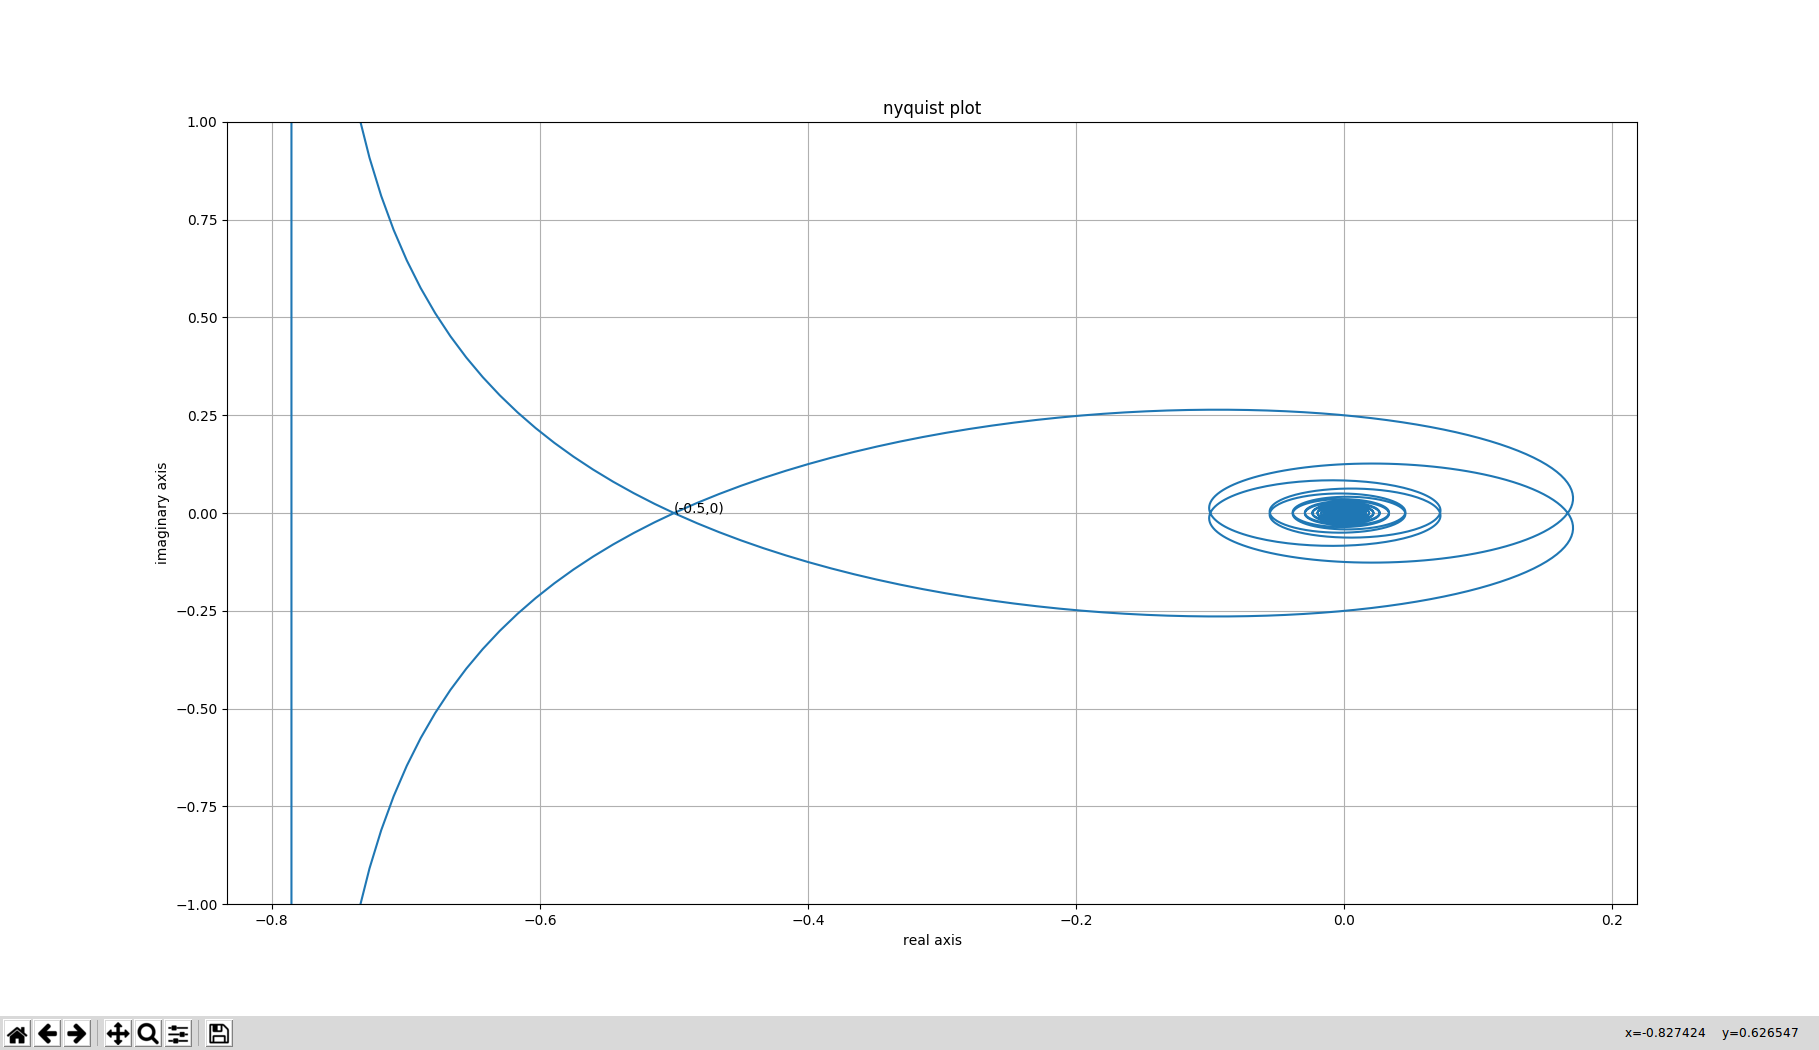
\includegraphics[width=\linewidth]{nyquist.eps}
  \caption{Nyquist plot}
  \label{fig:Nyquist plot}
\end{figure}
\\
\newline \textbf{Nyquist Stability Criterion} - for  the stability of a closed loop transfer function G(s)/(1+G(s)*H(s)) ,the number of poles of G(s)*H(s) on right half of s-plane must equal the number of encirclement of nyquist contour of  G(s)*H(s) about the critical point -1+0j
\\
\newline we must find
\begin{align}
Z=P-N    
\end{align}
\
Z=number of poles of closed loop transfer function in right half of s-plane.
\\ 
\newline P=number of poles of G(s)*H(s) in right half of s-plane
\\ 
\newline N=number of encirclement of nyquist contour of G(s)*H(s) about the critical point -1+0j,
here H(S)=1.
\\ 
\newline from plot we get N=0,and we already know P=0 since our G(s) doesnt have any poles on right half of s-plane
\begin{align}
Z=0-0=0
\end{align}
Z=0 implies the system is stable because we dont have any poles on right half of the s-plane



\end{enumerate}
